\documentclass[11pt]{scrartcl}
\usepackage[sexy]{evan}
\usepackage{graphicx}

\newcommand{\N}{\mathbb{N}}
\newcommand{\Z}{\mathbb{Z}}
\newcommand{\F}{\mathbb{F}}
\newcommand{\Q}{\mathbb{Q}}
\newcommand{\R}{\mathbb{R}}
\newcommand{\C}{\mathbb C}


\newcommand{\Vu}{\mathbf{u}}
\newcommand{\Vv}{\mathbf{v}}
\newcommand{\Vw}{\mathbf{w}}
\newcommand{\Vx}{\mathbf{x}}
\newcommand{\Ve}{\mathbf{e}}
\newcommand{\Vc}{\mathbf{c}}
\newcommand{\Vb}{\mathbf{b}}



\newcommand{\Va}{\mathbf{a}}

\newcommand{\Vhx}{\mathbf{\hat{x}}}

\newcommand{\Vy}{\mathbf{y}}
\newcommand{\Vz}{\mathbf{z}}
\newcommand{\Vo}{\mathbf{0}}

%From Topology
\newcommand{\cT}{\mathcal{T}}
\newcommand{\cB}{\mathcal{B}}
\newcommand{\cC}{\mathcal{C}}

\usepackage{answers}
\Newassociation{hint}{hintitem}{all-hints}
\renewcommand{\solutionextension}{out}
\renewenvironment{hintitem}[1]{\item[\bfseries #1.]}{}
\declaretheorem[style=thmbluebox,name={Theorem}]{thm}

\begin{document}
\title{CS 182}
\author{Vishal Raman}
\thispagestyle{empty}
$ $
\vfill
\begin{center}

\centerline{\huge \textbf{CS 182 Lecture Notes, Spring 2022}}
\centerline{\Large \textbf{Deep Learning} } 
\centerline{Professor: Marvin Zhang}
\centerline{Vishal Raman}
\end{center}
\vfill
$ $
\newpage
\thispagestyle{empty}
\tableofcontents
\newpage
%\maketitle
\section{02/28/2022 - Recurrent Neural Networks}
\subsection{Problem Setup}
We consider settings in which the features $\textbf{x}$ represent \textit{sequential data} which may be \textbf{variable length}. Some examples include
\begin{itemize}
\item Text of different lengths
\item Audio recordings/waves
\item Video recordings
\end{itemize} 
The labels could be scalars $y$(sentiment analysis, identification), or they could be sequences $\textbf{y}$(translation, transcription, captioning).  There could also be 
no label at all!  This is true in unsupervised learning/generating modeling.

Some models we use include:
\begin{itemize}
\item Markov/n-gram models, hidden Markov models(HMMs)
\item Embedding/clustering-based methods
\item Convolutions("temporal" convolutions which could be a 1-d convolution of a sequence, or a 3-d convolution over a video).
\item Recurrent Neural Networks(RNNs)
\item Long short-term memory(LSTM)
\item Gated Recurrent Units(GRUs)
\item Transformers
\end{itemize}

\subsection{Dealing with Variable Length Inputs}
Before, when dealing with images, we could reasonably assume fixed size inputs.  However, with sequential data, it can be assumed that the input lengths will almost always vary. 
\begin{center}
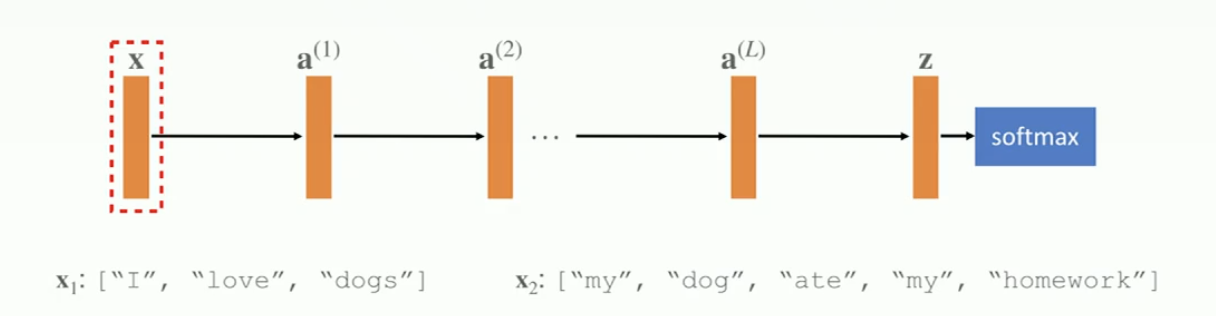
\includegraphics[scale=0.5]{images/var_length.png}
\end{center}

To deal with this, we feed one piece of input called a \textbf{token} per layer. 
\begin{center}
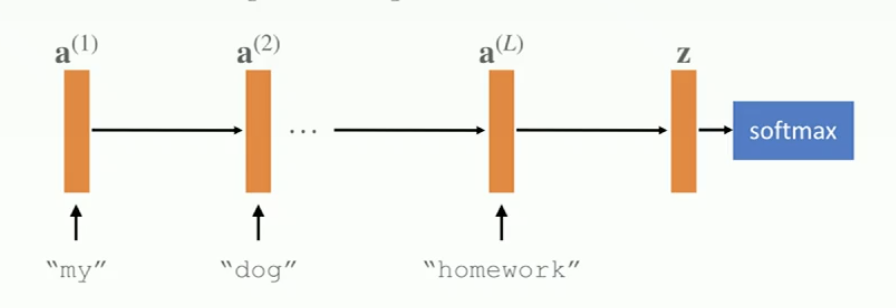
\includegraphics[scale=0.5]{images/token.png}
\end{center}
Now, the input to layer $\ell + 1$ is $[a^{(\ell)}; x[\ell] ]$.

The issues with this approach are the following:
\begin{itemize}
\item We need as many layers as the max number of tokens.  For very large inputs, we would have extremely deep networks which are difficult to train.
\item We have a different $W^{(\ell)}$ and $b^{(\ell)}$ for each layer, which is a massive number of items to optimize.  
\item The later layers get trained very rarely, so it's hard to generalize to longer sequences at test time.  
\item Another issue is that $a^{(1)}$ is missing the previous layer output. 
\end{itemize}
\subsection{Recurrent Neural Networks}
To solve some of these issues, we use \textbf{weight sharing}: use the same parameters in every layer.
$$\text{Before: } a^{(l + 1)} = \sigma(W^{(l + 1)}[a^{(l)}; x[l]] + b^{(l + 1)})$$
$$\text{Now: } a^{(l + 1)} = \sigma(W[a^{(l)}; x[l]] + b)$$

\begin{remark} In backpropagation, $W$ and $b$ get a gradient signal from every single time they are applied in the network, and we sum them to get the final gradient for $W$ and $b$.
\end{remark}

To address the problem with $a^{(1)}$, initialize some $a^{(0)}$ independently from the input $x$ and feed it into $a^{(1)}.$

Putting these two ideas together gives us the Recurrent Neural Network(RNN).

\begin{remark} The values $x[l]$ are encoded from some word2vec algorithm and the end vector is the same length for each word.
\end{remark}
\
The above applies for a sequence input, single output.  If we wanted sequence input, sequence output, we could output a scalar at each layer to get a sequence output.
\begin{center}
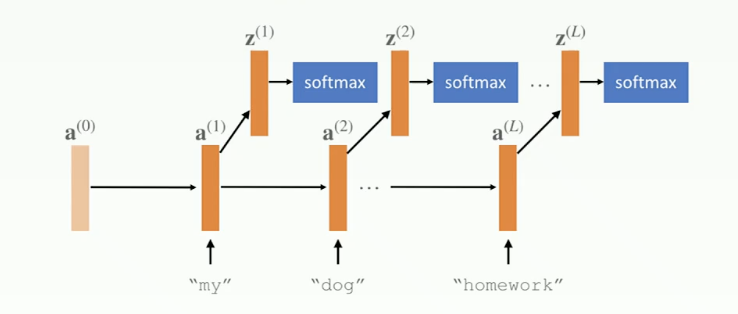
\includegraphics[scale=0.8]{images/seqout.png}
\end{center}

In general, different applications give rise to different ways we use RNNs.

\begin{center}
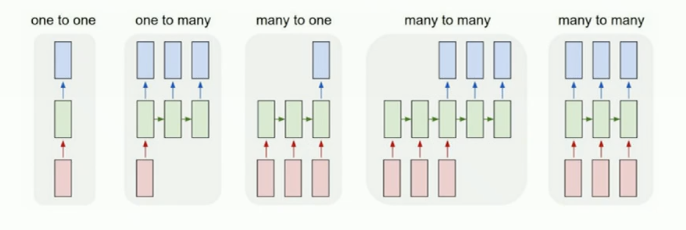
\includegraphics[scale=0.8]{images/atob.png}
\end{center}
\begin{itemize}
\item One-to-one is not an RNN.  It is like the ConvNet or Fully-Connected Net we have worked with.
\item For translation, we might do something like the 4th diagram, since we need to see the whole sentence before we can translate.
\item Image Captioning is single input, sequence output.
\item Sentiment Analysis is many to one, sequence input single output.
\item Text generation would be many to many like the last diagram.  
\item The many-to-many can have many different styles depending on the application.
\end{itemize}

\subsection{Generating Outputs from RNNs}
Generating a sequential output is done in an \textbf{autoregressive} manner: condition the model on what you have seen before to generate the next thing. 
\begin{center}
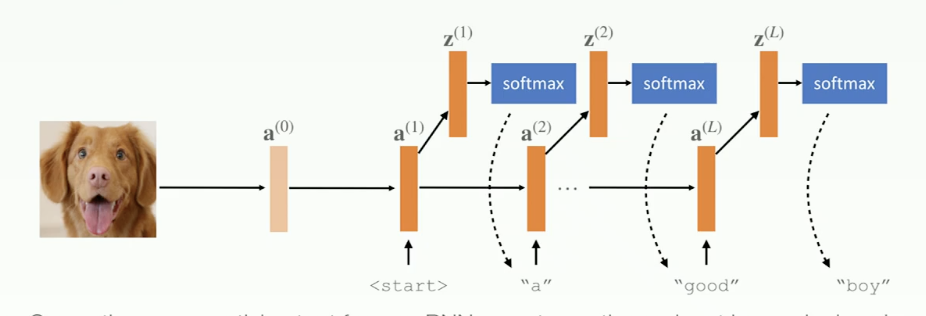
\includegraphics[scale=0.8]{images/autoreg.png}
\end{center}
\begin{remark} In the above, we assume that the RNN is already trained, and then we use it to generate text using the above scheme. 
\end{remark}

\subsection{Vanishing/Exploding Gradients}
What is the gradient of the final loss with respect to $W/b$?
\begin{center}
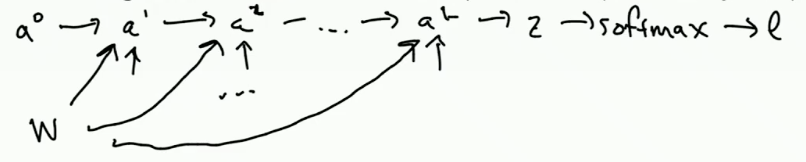
\includegraphics[scale=0.8]{images/grad.png}
\end{center}

We have 
$$\frac{d\ell}{dW} = \sum_{k=1}
^L \frac{d\ell}{da^k} \frac{da^k}{dW},$$
$$\frac{d\ell}{da^{1}} = \frac{d\ell}{da^L} \frac{da^L}{da^{L-1}} \dots \frac{da^2}{da^1},$$
so it is very easy for gradients to vanish or explode.

We can deal with this as follows:
\begin{itemize}
\item For exploding gradients, we can just \textbf{clip} the gradients - divide by the magnitude of the large gradients to make them smaller.
\item Vanishing gradients seem to require clever architecture choices: one idea we can use to address this is a \textbf{skip connection}!  
\item One architecture that does this is the \textbf{LSTM}: it is much older than skip-connections but employs the same basic principle that allow better gradient flow by making smarter connection choices. 
\end{itemize}
\section{Long Short-Term Memory(LSTM)}
\begin{center}
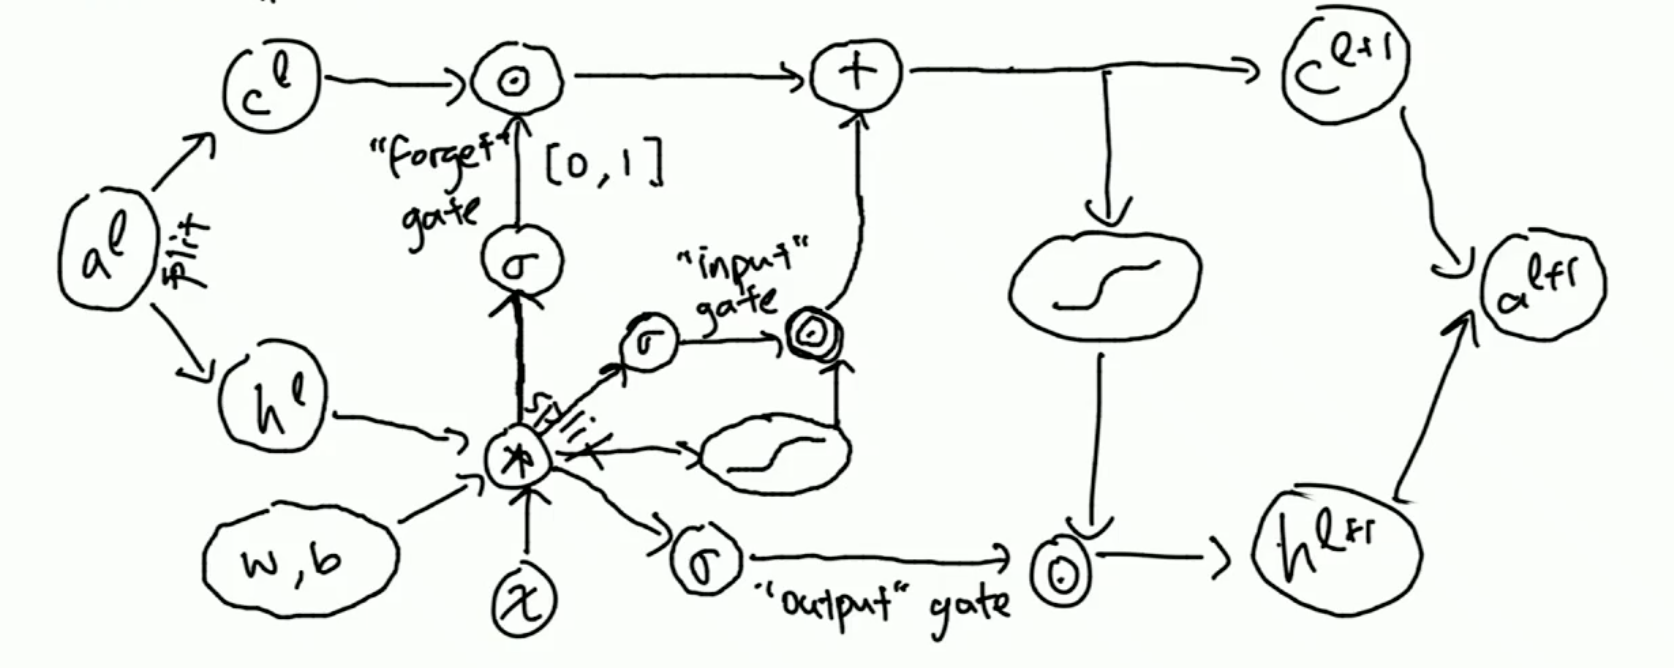
\includegraphics[scale=0.5]{images/lstm.png}
\end{center}

\begin{enumerate}
\item Start with a state $a^{\ell}$ and split into two states, $c^\ell$ the cell state, and $h^{\ell}$ the hidden state.  We have $d_{c} = d_h$, and $d_a = d_c + d_h$, since we exactly split $a$ into two parts. 
\begin{itemize}
\item $c^\ell$ is the part that acts like a skip so we have better gradient flow with long sequences.  
\item $h^\ell$ deals with the nonlinearities which we need for expressivity. 
\end{itemize}
\item For the cell state $c^\ell$, we element-wise multiply by scalars $f^\ell$ in $[0, 1]$(we can do this by passing some number into the sigmoid $\sigma$).  This is the \textbf{forget gate} - when the scalar is close to $0$, we forget these dimensions, and when the scalars are close to $1$, we retain the information and gradient flow.  Then, we add a bias $i^\ell$, which is called the \textbf{input} to the cell state.  This gives us $c^{\ell + 1}$.  Overall, we have 
$$c^{\ell + 1} = c^{\ell} \odot f^{\ell} + i^\ell.$$
\item For the hidden state $h^\ell$, we use an affine transformation using parameters $W, b$ and the input $x$.  This is split into $4$ equal parts each with the same dimension as $h$:
\begin{itemize}
\item The first piece determines $f^\ell$, the element sent into the \textbf{forget gate}.
\item The next piece is sent to a nonlinearity(doesn't matter which one) and a piece sent to the sigmoid which is elementwise-multiplied to the nonlinearity output.  This is called the \textbf{input gate}.
\item The last piece is sent to a sigmoid to be used for the output gate.
\end{itemize}
\item We also take $c^{l+1}$ and use a nonlinearity(doesn't matter which one) and element-wise multiplied by the component from the output gate to determine $h^{l+1}$.
\end{enumerate}

\begin{remark} Some elements are important but others are pretty arbitrary.  For example, the GRU is very similar but it doesn't have an output gate.  However, it still performs pretty well.
\end{remark}
\end{document}
